\section{SA³: Semantic Activity Annotation Algorithm}
\label{sec:clustering:sa3}

%Brief introduction to the algorithm:
%- Inspired in knowledge-driven techniques, specially in Chen's work
%- It is not activity recognition, but offline annotation
The objective of the $SA^3$ algorithm is to find sequences of actions that are describing an activity in an unlabelled sensor activation dataset. For that purpose, initial activity models (IAM) stored in the context knowledge are used. Remember that IAMs, as defined in definition \ref{def-iam}, are characterised by a sequence of necessary actions to perform an activity plus a duration estimation. 

The problem can be stated more formally as:

\begin{problem}[$SA^3$]
\label{prob-sa3}
 Given a context knowledge file where activities, sensors and objects are described and an unlabelled sensor activation dataset, find the occurrences of IAMs that form a valid execution of an activity.
\end{problem}

Considering that IAMs are sequences of actions and that sensor activation datasets are sensor sequences, Problem \ref{prob-sa3} can be seen as a pattern recognition problem, where IAMs act as the patterns to be recognised in the sensor activation dataset. Although $SA^3$ is actually a pattern recognition algorithm, there are some important features that make the problem special. Namely:

\begin{itemize}
 \item IAMs are sequences of actions, whereas sensor activation datasets contain sensor activations, i.e. the activation of a concrete sensor of the environment.
 \item As IAMs are incomplete activity models, a sensor activation dataset will generally include sensor activations that are interleaved with IAMs in the same activity.
 \item IAMs have no information about the order in which actions are executed, thus if $IAM(A) = \{a, b, c\}$, a sensor activation dataset containing the sequence $\{c, a, b\}$ has to be identified as activity $A$, i.e. the elements of the pattern to be recognised might appear in varied orders.
 \item Even though a sequence corresponding to an IAM is found, it does not necessarily describe a valid activity, since duration and location are important. For example, for an activity whose typical duration is 5 minutes, corresponding actions are found but their distance is of 3 hours; it is then common sense to think that those actions do not form a valid activity. Hence, the pattern recognition algorithm needs to take action time distances and locations into account.
 \item Sensors are prone to errors and in consequence, sensor activation datasets contain noise. The pattern recognition algorithm has to work thus in noisy environments. More concretely, considered kinds of sensor noise are positive and missing sensor noise (definitions \ref{def-positive} and \ref{def-missing}).
\end{itemize}

In summary, $SA^3$ has to use IAMs as patterns to be recognised in an unlabelled sensor activation dataset, where actions are executed in varied orders, where actions that are not in IAMs can appear interleaved, where duration and location information is crucial for the validity of a pattern and where sensor noise exists. 

In order to tackle Problem \ref{prob-sa3} a three-step algorithm has been designed and implemented (see Figure \ref{fig:sa3_algorithm}). The first step, named sensor-action transformation step, uses sensor information from the context knowledge to transform sensor activations into actions (Section \ref{subsec:clustering:sa3:transform}). The second step, the activity sequence finding step, runs a pattern recognition algorithm using IAMs and object information from context knowledge, as described in Section \ref{subsec:clustering:sa3:find}. This step addresses the varied order of actions, interleaved actions not pertaining to IAMs, duration and location information for valid activities and sensor noise. Finally, the third step called correct activity sequence fitting fixes the overlapping activities generated in the second step (Section \ref{subsec:clustering:sa3:fit}).

\begin{figure}[htbp]
\centering
\includegraphics[width=\textwidth]{sa3_algorithm.pdf}
    \caption{The three-step algorithm for $SA^3$.}
    \label{fig:sa3_algorithm}
\end{figure}

The result of $SA^3$ is the partially annotated dataset. $SA^3$ can only label those actions pertaining to IAMs and thus it cannot infer a label for all the other actions of the sensor activation dataset. An example of how a partially annotated dataset looks like is provided in Figure \ref{fig-partially-annotated}. The first column shows the time-stamp of the sensor activation. The second column shows the activated sensor. Those two columns form the sensor activation dataset. $SA^3$ adds the third, fourth and fifth columns, where action, activity label and start/end tags are provided. Start tag refers to the first action of the IAM of detected activity detected in a valid activity discovered by $SA^3$. End tag has the same meaning but for the last action. In consequence, start and end tags show the start and end times for a detected activity. For convenience, and even though any action not pertaining to the IAM of the detected activity cannot be labelled by $SA^3$, all the actions between start and end times are labelled with the detected activity name, and not with the special label 'None'. This labelling criterion is applied to make visualization easier and it does not have any effect on the output of $SA^3$, neither for $AC$ nor for evaluation purposes.

\begin{figure}[htbp]
\begin{small}
\begin{lstlisting}
2014-05-23 07:42:17.106962,wsugarSens,hasFlavour,None,
2014-05-23 07:49:17.310460,bedSens,useFurniture,None,
2014-05-23 09:43:44.128079,cupSens,hasContainer,MakeChocolate,start
2014-05-23 09:47:33.984341,storeSens,openStore,MakeChocolate,
2014-05-23 09:47:39.333528,potSens,useCookingUtensil,MakeChocolate,
2014-05-23 09:47:52.750216,cookerSens,useCookingAppliance,MakeChocolate,
2014-05-23 09:48:07.764138,fridgeSens,openFridge,MakeChocolate,
2014-05-23 09:48:12.591836,wmilkSens,hasMilk,MakeChocolate,
2014-05-23 09:48:47.199512,chocoSens,hasChocolate,MakeChocolate,end
2014-05-23 09:54:11.553695,mugSens,hasContainer,None,
\end{lstlisting}
\end{small}
\caption{Example of a partially annotated dataset, the output of the $SA^3$ algorithm.}
\label{fig-partially-annotated}
\end{figure}


% Note: The following two paragraphs can be used in summary and conclusions?
%Real-time activity recognition needs complete activity models to have a reliable recognition performance. However, providing complete activity models is very complicated, since each user executes varied action sequences to perform the same activity. For example, to make a coffee, some users may use milk and sugar, while others may add only some cream. But making coffee will always imply using coffee and having a container, i.e. the action sequence \textit{\{hasContainer(x), hasCoffee(y)\}}. This prior knowledge is used in $SA^3$ for activity annotation.

%Activity annotation and recognition is not the same thing. Activity annotation can make use of the whole dataset offline, with no time restrictions. On the other hand, activity recognition is required to work while activities are being performed, so only past sensor activations can be used. This key difference makes feasible using incomplete activity models to annotate activities, in contrast with the real-time recognition problem.

\subsection{Sensor-action transformation step}
\label{subsec:clustering:sa3:transform}

The first step takes as inputs the sensor activation dataset and the context knowledge file to transform every sensor activation into an action. For each sensor activation in the dataset, the corresponding sensor model is checked in the context knowledge file. As shown in Figure \ref{fig-context-json} every sensor has the action to which it has to be mapped in the context knowledge file provided by the domain expert. This simple transformation is possible due to the dense sensing-based activity monitoring approach, where sensor activations are directly linked to user-object interactions and thus to actions. 

In consequence, a sensor activation sequence such as:
 \begin{equation*}
 \begin{split}
   \{cupObjSensor, whiteSugarSensor, skimmedMilkSensor\}
 \end{split}  
 \end{equation*}
 will be transformed to:
 \begin{equation*}
 \begin{split}
  \{hasContainer(cup), hasFlavour(white\text{-}sugar), hasMilk(skimmed\text{-}milk)\}
 \end{split}   
 \end{equation*}
 
For the sake of clarity, and given that action matching does not care about concrete objects used to execute that action, \textit{hasContainer(cup)} will be used as \textit{hasContainer}. But notice that the object information obtained through the sensor activation is not removed. 

Sensor-action transformation step allows performing pattern recognition in the action space, abstracting from concrete sensor activations. This step can be kept simple thanks to the dense sensing-based approach. For different activity monitoring approaches, such as wearable sensors, more complex sensor-action transformation steps should be implemented. However, notice that as far as sensor information can be transformed to actions, $SA^3$ and the entire clustering process can work without problem. This is why constraint \ref{cons-dense} is considered a weak constraint.

\subsection{Activity sequence finding step}
\label{subsec:clustering:sa3:find}

All the occurrences of minimal activity models are found iterating on the action dataset. For an action pertaining to a minimal activity model following actions are searched. Those actions are considered to describe the activity if two criteria are fulfilled: 
 \begin{enumerate}
  \item \textit{Completion criterion}: the action sequence has to contain all the actions of the corresponding minimal activity model
  \item \textit{Duration criterion}: the duration of the action sequence has to be smaller than the duration estimation of the corresponding minimal activity model
  \item \textit{Location compatibility criterion}:
 \end{enumerate}
 Depending on the activity models, the actions dataset and noise levels, detected activities can overlap each other. Here is an illustrative example, where time-stamps are ignored since duration criterion is satisfied. Imagine we define minimal activity models for \textit{MakeCoffee, MakeTiramisu, MakeWhippedCream} and \textit{BrushTeeth}, where:
 \begin{equation*}
  \begin{split}
   MakeCoffee =\{hasCoffee, hasContainer, hasFlavour\} \\
  MakeTiramisu = \{hasCream, hasContainer, hasCoffee\} \\
  MakeWhippedCream = \{hasFlavour, hasContainer, hasCream\} \\
  BrushTeeth = \{hasBrusher, hasToothPaste, turnOnTap\} 
  \end{split}
 \end{equation*} 
 
Let us consider the following action sequence from the action dataset:
\begin{equation*}
\begin{split}
 \{hasContainer, hasCream, useCookingUtensil, hasFlavour, hasBrusher, \\ 
 hasCoffee, hasToothPaste, hasContainer, turnOnTap\}
\end{split}  
\end{equation*}
Figure \ref{fig:overlap} shows all the activities found applying the completion and duration criterion. Activities overlap each other, because there are several actions that belong to several activities. Notice also that there are some actions that are not in any activity model, which is totally feasible for our approach.
\begin{figure}[htbp]
\centering
\includegraphics[width=\textwidth]{overlapping_activities.pdf}
    \caption{Illustrative example of the output of the step 2 of $SA^3$. MWC refers to \textit{MakeWhippedCream}, MT to \textit{MakeTiramisu}, MC to \textit{MakeCoffee} and BT to \textit{BrushTeeth}}
    \label{fig:overlap}
\end{figure}

\subsection{Correct activity sequence fitting step}
\label{subsec:clustering:sa3:fit}
Having the overlapping activities, the objective of this step is to find the maximum number of activities that do not overlap. This heuristic is derived from the fact that only none interleaved activities are considered. Applying it, the example of Figure \ref{fig:overlap} can be solved appropriately. The solution found by the algorithm is that there are only two activities in that action sequence:
\begin{equation*}
  \begin{split}   
  MakeWhippedCream = \{hasContainer, hasCream, useCookingUtensil, hasFlavour\} \\
  BrushTeeth = \{hasBrusher, hasCoffee, hasToothPaste, hasContainer, turnOnTap\} 
  \end{split}
 \end{equation*}  

Hence, \textit{hasCoffee} is probably due to a faulty sensor activation and \textit{hasContainer} may refer to a glass used in the bathroom to rinse the mouth. 

\subsection{The complete SA³ algorithm}


This three-step algorithm is depicted as pseudo-code in Algorithm \ref{alg:sa3}. It has been designed to work with noisy sensor activations, varying order for activity executions and sensor activations that do not belong to any activity model. That flexibility allows using the tool in many different datasets. Section \ref{evaluation} contains many cases to show the performance of the algorithm in several demanding situations.

\begin{algorithm}
 \caption{$SA^3$ algorithm for semantic activity annotation}
 \label{alg:sa3}
 \begin{algorithmic}
 \REQUIRE sensor\_dataset, transformation\_function, minimal\_activity\_models
 \ENSURE annotated\_dataset
 \STATE $action\_dataset \leftarrow apply\_transform\_function(sensor\_dataset, transformation\_function)$
 \FORALL{$action \in action\_dataset$}
  \IF{$action \in minimal\_activity\_models$}    
    \STATE $activities \leftarrow obtain\_activities(action, minimal\_activity\_models)$
  \ENDIF
  \FORALL{$activity \in activities$}
    \STATE $// \text{ Use duration and completion criteria}$
    \STATE $detected\_activities \leftarrow find\_proper\_activities(minimal\_activity\_models)$
  \ENDFOR
 \ENDFOR
 \STATE $annotated\_dataset \leftarrow find\_non\_overlapping\_activities(detetected\_activities)$
 \RETURN $annotated\_dataset$
 \end{algorithmic}
\end{algorithm}
